%%%%%%%%%%%%%%%%%%%%%%%%%%%%%%%%%%%%%%%%%%%%%%%%%%%%%%%%%%%%
%%%%%%%%%%%%%%%%%%%%%%%%%%%%%%%%%%%%%%%%%%%%%%%%%%%%%%%%%%%%
%%%%%%%%%%%%%%%%%%%%%%%%%%%%%%%%%%%%%%%%%%%%%%%%%%%%%%%%%%%%
\section{More on Constrained Function Spaces}\label{Sec:ConstrainedSpaces}
%%%%%%%%%%%%%%%%%%%%%%%%%%%%%%%%%%%%%%%%%%%%%%%%%%%%%%%%%%%%
%%%%%%%%%%%%%%%%%%%%%%%%%%%%%%%%%%%%%%%%%%%%%%%%%%%%%%%%%%%%
%%%%%%%%%%%%%%%%%%%%%%%%%%%%%%%%%%%%%%%%%%%%%%%%%%%%%%%%%%%%

\subsection{How to Construct Constrained Spaces}

As we have seen we often have the situation that problems have to be solved in a
subspace $\tilde{U}_h\subset U_h$ or even an affine subspace
$w_h+\tilde{U}_h$, where $w_h\in U_h$.

\paragraph{Basis transformation} 

\begin{frame}
\frametitle<presentation>{Basis Transformation}
\begin{Def}[Basis Transformation] Consider an alternative basis
$\Phi_{U_h}'=\{\phi_i'\,|\, i\in \mathcal{I}_{U_h}\}$ of $U_h$
obtained by
\begin{equation}
\phi_i' = \sum_{j\in\mathcal{I}_{U_h}}
\left(\mathbf{T}_{U_h}\right)_{i,j} \phi_j, \qquad i\in \mathcal{I}_{U_h}.
\end{equation}
$\mathbf{T}_{U_h}$ is the \textit{transformation matrix}.\hfill$\square$
\end{Def}
For $\mathbf{U}'=\mathbb{K}^{\mathcal{I}_{U_h}}$ we have the isomorphism
$\text{FE}_{\Phi_{U_h}'}(\mathbf{u}') = \sum_{i\in\mathcal{I}_{U_h}}
(\mathbf{u}')_i \phi_i'$ and get
\begin{equation}
\begin{split}
u_h &= \text{FE}_{\Phi_{U_h}'}(\mathbf{u}') = 
\sum_{j\in\mathcal{I}_{\tilde{U}_h}} (\mathbf{u}')_j \phi'_j = 
\sum_{j\in\mathcal{I}_{U_h}} (\mathbf{u}')_j \left (
\sum_{i\in\mathcal{I}_{U_h}}
\left(\mathbf{T}_{U_h}\right)_{j,i} \phi_i \right)\\
&= \sum_{i\in \mathcal{I}_{U_h}} \left (\sum_{j\in\mathcal{I}_{U_h}}
\left(\mathbf{T}^T_{U_h}\right)_{i,j} (\mathbf{u}')_j \right ) \phi_i
= \text{FE}_{\Phi_{U_h}}\left( \mathbf{T}^T_{U_h} \mathbf{u}' \right) .
\end{split}
\end{equation}
\end{frame}

\paragraph{Splitting and Subspaces} 

\begin{frame}
\frametitle<presentation>{Splitting and Subspaces}
Subspaces are introduced by a splitting of
the index set into unconstrained and constrained indices:
\begin{equation*}
\mathcal{I}_{U_h} = \tilde{\mathcal{I}}_{U_h} \cup
\bar{\mathcal{I}}_{U_h}, \qquad  \tilde{\mathcal{I}}_{U_h} \cap
\bar{\mathcal{I}}_{U_h} = \emptyset.
\end{equation*}
With respect to this splitting we define the subspaces
\begin{align*}
\tilde{U}_h' &= \text{span}\ \{\phi_i'\,|\,
i\in\tilde{\mathcal{I}}_{U_h}\}, &
\bar{U}_h' &= \text{span}\ \{\phi_i'\,|\,
i\in\bar{\mathcal{I}}_{U_h}\}
\end{align*}
and the corresponding coefficient spaces
\begin{align*}
\tilde{\mathbf{U}}' &=
\mathbb{K}^{\tilde{\mathcal{I}}_{U_h}}, &
\bar{\mathbf{U}}' &=
\mathbb{K}^{\bar{\mathcal{I}}_{U_h}}.
\end{align*}

$\tilde{U}_h := \tilde{U}_h'\subseteq U_h$ is the desired subspace of
$U_h$ where we want to solve the constrained problem.
\end{frame}


\begin{frame}
\frametitle<presentation>{Simplified Transformation Matrix}
The transformation matrix $\mathbf{T}_{U_h}$ is written in block
form w.r.t. the splitting:
\begin{equation*}
\mathbf{T}_{U_h} = \left(\begin{array}{cc}
\mathbf{T}_{\tilde{U}_h,\tilde{U}_h} & \mathbf{T}_{\tilde{U}_h,\bar{U}_h}\\
\mathbf{T}_{\bar{U}_h,\tilde{U}_h} & \mathbf{T}_{\bar{U}_h,\bar{U}_h}
\end{array}\right) .
\end{equation*}
We show below that it suffices to consider transformations of the form
\begin{equation}\label{Eq:StructureTransformation}
\mathbf{T}_{U_h} = \left(\begin{array}{cc}
\mathbf{I} & \mathbf{T}_{\tilde{U}_h,\bar{U}_h}\\
\mathbf{0} & \mathbf{I}
\end{array}\right)
\end{equation}
which means transformations have the form
\begin{equation*}
\phi_i' = \phi_i + \sum_{j\in\bar{\mathcal{I}}_{U_h}}
\left(\mathbf{T}_{\tilde{U}_h,\bar{U}_h}\right)_{i,j} \phi_j, \qquad i\in \tilde{\mathcal{I}}_{U_h}.
\end{equation*}
The $\tilde{\mathcal{I}}_{U_h} \times \bar{\mathcal{I}}_{U_h}$  matrix
$\mathbf{T}_{\tilde{U}_h,\bar{U}_h}$ will usually be very sparse (or
even zero).
\end{frame}

\paragraph{Restrictions} 

\begin{frame}<article>
\frametitle<presentation>{Restriction Operators}
Below we will make use of the following restriction operators
\begin{align*}
\mathbf{R}_{\tilde{\mathbf{U}}',\mathbf{U}'} &: \mathbf{U}' \to \tilde{\mathbf{U}}', & 
(\mathbf{R}_{\tilde{\mathbf{U}}',\mathbf{U}'}\mathbf{u}')_i &= 
(\mathbf{u}')_i \quad \forall i\in \tilde{\mathcal{I}}_{U_h},\\
\mathbf{R}_{\bar{\mathbf{U}}',\mathbf{U}'} &: \mathbf{U}' \to \bar{\mathbf{U}}', & 
(\mathbf{R}_{\bar{\mathbf{U}}',\mathbf{U}'}\mathbf{u}')_i &= 
(\mathbf{u}')_i \quad \forall i\in \bar{\mathcal{I}}_{U_h}.
\end{align*}

Note that $\mathbf{Q}_{\tilde{\mathbf{U}}}
= \mathbf{R}_{\tilde{\mathbf{U}}',\mathbf{U}'}^T \mathbf{R}_{\tilde{\mathbf{U}}',\mathbf{U}'}$
is an orthogonal projection.

It can be used to project a function from $U_h$ to $\tilde{U}_h$ as
follows:
\begin{align*}
P_h &: U_h \to \tilde{U}_h, & P_h  =
FE_{\Phi_h'} \circ \mathbf{Q}_{\tilde{\mathbf{U}}} \circ
FE_{\Phi_h'}^{-1} .
\end{align*}

The projection $P_h$ will play a major role below.
\end{frame}

\subsection{Examples of Constrained Spaces}

\paragraph{Dirichlet Boundary Conditions}

\begin{frame}
\frametitle<presentation>{Dirichlet Boundary Conditions}
$U_h^1$ :  piecewise-linear, conforming finite
element functions.

$\tilde{U}_h^1 = \{u\in U_h^1 \,|\, \text{``$u(x)=0$'' for
$x\in \Gamma_D$}\}$.

Then just set 
\begin{align*}
\bar{\mathcal{I}}_{U_h} &= \{i\in \mathcal{I}_{U_h} \,|\,
x_{z_i}\in\Gamma_D\}, &
\tilde{\mathcal{I}}_{U_h} =  \mathcal{I}_{U_h}\setminus\bar{\mathcal{I}}_{U_h}
\end{align*}
and
\begin{equation*}
\phi_i' = \phi_i \qquad i\in \tilde{\mathcal{I}}_{U_h}.
\end{equation*}

Obviously, $\mathbf{T}_{\tilde{U}_h,\bar{U}_h}=\mathbf{0}$ in this case.
\end{frame}

\paragraph{Hanging Nodes}

Consider a mesh obtained from non-conforming refinement.

\begin{frame}
\frametitle<presentation>{Hanging Nodes}
\begin{columns}
\begin{column}{0.6\textwidth}
$U_h^1$ now is the space of piecewise linear functions with degrees of
freedom in \textit{all} vertices of the mesh. \\
\medskip
To obtain the subspace $\tilde{U}_h^1 = U_h^1 \cap C^0(\Omega)$ we set 
\begin{align*}
\bar{\mathcal{I}}_{U_h} &= \{i\in \mathcal{I}_{U_h} \,|\, \text{$z_i$ is a
hanging node} \}, \\
\tilde{\mathcal{I}}_{U_h} &=  \mathcal{I}_{U_h}\setminus\bar{\mathcal{I}}_{U_h}.
\end{align*}
\end{column}
\mode<presentation>{
\begin{column}{0.4\textwidth}
\psfrag{0}{{\tiny $0$}}
\psfrag{1}{{\tiny $1$}}
\psfrag{h}{{\tiny $\frac12$}}
\psfrag{vi}{$v_i$}
\psfrag{vj}{$v_j$}
\psfrag{vk}{$v_k$}
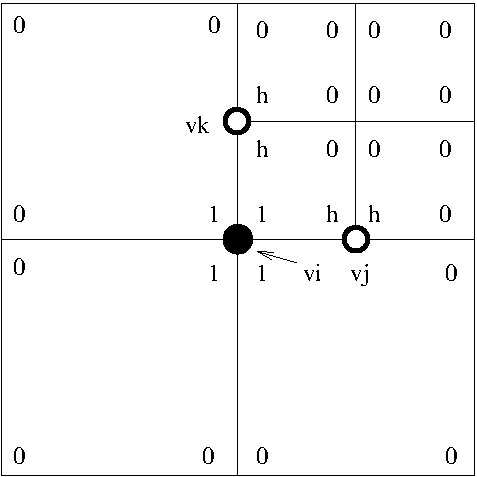
\includegraphics[width=\textwidth]{./EPS/function3}
\end{column}}
\end{columns}
\mode<article>{
\begin{figure}
\begin{center}
\psfrag{0}{{\tiny $0$}}
\psfrag{1}{{\tiny $1$}}
\psfrag{h}{{\tiny $\frac12$}}
\psfrag{vi}{$v_i$}
\psfrag{vj}{$v_j$}
\psfrag{vk}{$v_k$}
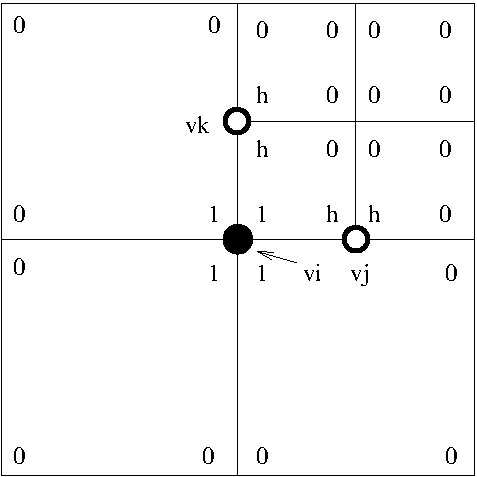
\includegraphics[width=0.5\textwidth]{./EPS/function3}
\end{center}
\caption{Non-conforming refinement and piecewise linear finite elements.}
\end{figure}}
For the vertex $i$ in the figure we obtain, e.~g., the basis function
\begin{equation*}
\phi_i' = \phi_i + \frac12 \phi_j + \frac12 \phi_k .
\end{equation*}
\end{frame}


\paragraph{Pure Neumann Problem}

\begin{frame}<article>
\frametitle<presentation>{Pure Neumann Problem}
We wish to solve
\begin{align*}
                -\Delta u &= f& \text{in }& \Omega\subseteq\mathbb{R}^n,\\
     - \nabla u\cdot\nu   &= j& \text{on }& \partial\Omega
\end{align*}
where $\int_{\partial\Omega} j \, ds = \int_\Omega f \, dx$.

Again, consider $U_h^1$, the piecewise-linear, conforming finite
element functions.

Then $u$ is only defined up to a constant and we wish to solve in
\begin{equation*}
\tilde{U}^1_h = \left\{u \in U^1_h \,\Biggl |\, \int_\Omega u \, dx = 0\right\}.
\end{equation*}

Set $\bar{\mathcal{I}}_{U_h}=\{0\}$, $\tilde{\mathcal{I}}_{U_h}
= \mathcal{I}_{U_h}\setminus\{0\}$ and
\begin{equation*}
\phi_i' = \phi_i - \frac{\int_\Omega\phi_i\, dx}{\int_\Omega\phi_0\,
dx} \phi_0, \qquad \forall i\in\tilde{\mathcal{I}}_{U_h}.
\end{equation*}
\end{frame}

\paragraph{Other Situations Where Constraints Occur}

\begin{frame}
\frametitle<presentation>{Other Constraints}
In addition to Dirichlet, hanging nodes and pure Neumann constraints we can also treat
\begin{itemize}
\item Varying polynomial degree in conforming finite elements
($p$-refinement).
\item Combination of $p$-refinement, non-conforming refinement and essential
boundary conditions.
\item Non-conforming refinement in mixed finite elements.
\item Periodic boundary conditions.
\item Constraints in parallel overlapping Schwarz methods.
\end{itemize}
\end{frame}


\subsection{Implementation of Dirichlet Constraints}

We now show how constraints can be added to a grid function space.

\begin{frame}
\frametitle<presentation>{Adding Constraints to a Grid Function Space}
Constraints are a property of a grid function space.

In addition to the local finite elements we have to
parametrize \lstinline{Dune::PDELab::GridFunctionSpace} with a type
that can provide the sparse transformation matrix
$\mathbf{T}_{\tilde{U}_h,\bar{U}_h}$ from \eqref{Eq:StructureTransformation}. 

Information should be provided only locally. One
column of $\mathbf{T}_{\tilde{U}_h,\bar{U}_h}$ may only involve
degrees of freedom of two (intersecting) elements.

A constraints class provides rows of
$\mathbf{T}^T_{\tilde{U}_h,\bar{U}_h}$ and may have methods
\begin{itemize}
\item \lstinline{volume}: Constrain degrees of freedom associated with
volume (useful in parallelization).
\item \lstinline{skeleton}: Constrain degrees of freedom associated
with interior intersections (useful for hanging nodes).
\item \lstinline{boundary}: Constrain degrees of freedom on boundary
intersections (for boundary conditions).
\end{itemize}
Flags \lstinline{do...} control which methods must be provided.
\end{frame}

\begin{onlyenv}<article>
  Depending on the type of the constraints, certain additional
  information are necessary,
  e.g. in the following example, the class \lstinline{Dune::PDELab::Q1Constraints} needs to know, if a
  given point on a boundary belongs to a Dirichlet boundary, or
  not. These information usually depend on the given problem and can
  differs for different components of the
  \lstinline{Dune::PDELab::GridFunctionSpace} tree.
\end{onlyenv}

\begin{frame}<presentation>[fragile,allowframebreaks,allowdisplaybreaks]
\frametitle<presentation>{Constraints Assembler Listing}
\framesubtitle<presentation>{File \texttt{src/course-gridfunctionspace/q1constraints.hh}}
\lstinputlisting[basicstyle=\scriptsize,numbers=left, 
numberstyle=\tiny, numbersep=5pt]{../../src/course-gridfunctionspace/q1constraints.hh}
\end{frame}
\mode<article>{
\begin{Lst}[File src/course-gridfunctionspace/q1constraints.hh] \mbox
\nopagebreak
\lstinputlisting[basicstyle=\scriptsize,numbers=left, 
numberstyle=\tiny, numbersep=5pt]{../../src/course-gridfunctionspace/q1constraints.hh}
\end{Lst}}

\begin{frame}
\frametitle<presentation>{A Boundary Condition Function}
To use assembling of constraints 
we have to provide the parameters required by the given type of
constraints.

In this example it must provide a method
\only<presentattion>{\begin{center}}
\lstinline{isDirichlet}
\only<presentattion>{\end{center}}
(see line \ref{bcp:name}), which is derived from
\only<presentattion>{\begin{center}}\only<article>{\newline}
\lstinline{Dune::PDELab::DirichletConstraintsParameters}
\only<presentattion>{\end{center}}
(see line \ref{bcp:base}). This class is defined in
\only<presentattion>{\begin{center}}\only<article>{\newline}
\texttt{dune/pdelab/constraints/constraintsparameters.hh}.
\only<presentattion>{\end{center}}
\end{frame}

\begin{frame}<presentation>[fragile,allowframebreaks,allowdisplaybreaks]
\frametitle<presentation>{Boundary Constraints Parameters Listing}
\framesubtitle<presentation>{File \texttt{src/course-gridfunctionspace/q1constraintsparameters.hh}}
\lstinputlisting[basicstyle=\scriptsize,numbers=left, 
numberstyle=\tiny, numbersep=5pt]{../../src/course-gridfunctionspace/q1constraintsparameters.hh}
\end{frame}
\mode<article>{
\begin{Lst}[File src/course-gridfunctionspace/q1constraintsparameters.hh] \mbox
\nopagebreak
\lstinputlisting[basicstyle=\scriptsize,numbers=left, 
numberstyle=\tiny, numbersep=5pt]{../../src/course-gridfunctionspace/q1constraintsparameters.hh}
\end{Lst}}

\begin{frame}
\frametitle<presentation>{Interpolation with Constraints}
In the following listing we redo the interpolation example 
with a constrained finite element space.

In line \ref{cint:newparameter} the grid function space is
parametrized with the constraints class.

In line \ref{cint:container} the grid function space exports a type to
hold the transformation matrix
$\mathbf{T}^T_{\tilde{U}_h,\bar{U}_h}$. 

In line \ref{cint:bcparam} the function giving the boundary
condition type is instantiated.

Finally, in line \ref{cint:constraints} the constraints are assembled
and stored.

Function \lstinline{Dune::PDELab::set_nonconstrained_dofs} in
line \ref{cint:setconstraints} allows to set all nonconstrained
degrees of freedom to a given value.

Function \lstinline{Dune::PDELab::set_constrained_dofs} does the same
for the constrained degrees of freedom.
\end{frame}


\begin{frame}<presentation>[fragile,allowframebreaks,allowdisplaybreaks]
\frametitle<presentation>{Constrained Interpolation Listing}
\framesubtitle<presentation>{File \texttt{src/course-gridfunctionspace/q1constrainedinterpolate.hh}}
\lstinputlisting[basicstyle=\scriptsize,numbers=left, 
numberstyle=\tiny, numbersep=5pt]{../../src/course-gridfunctionspace/q1constrainedinterpolate.hh}
\end{frame}
\mode<article>{
\begin{Lst}[File src/course-gridfunctionspace/q1constrainedinterpolate.hh] \mbox
\nopagebreak
\lstinputlisting[basicstyle=\scriptsize,numbers=left, 
numberstyle=\tiny, numbersep=5pt]{../../src/course-gridfunctionspace/q1constrainedinterpolate.hh}
\end{Lst}}

\begin{frame}<presentation>
\frametitle<presentation>{Visualization of Affine Shift Function}
\begin{center}
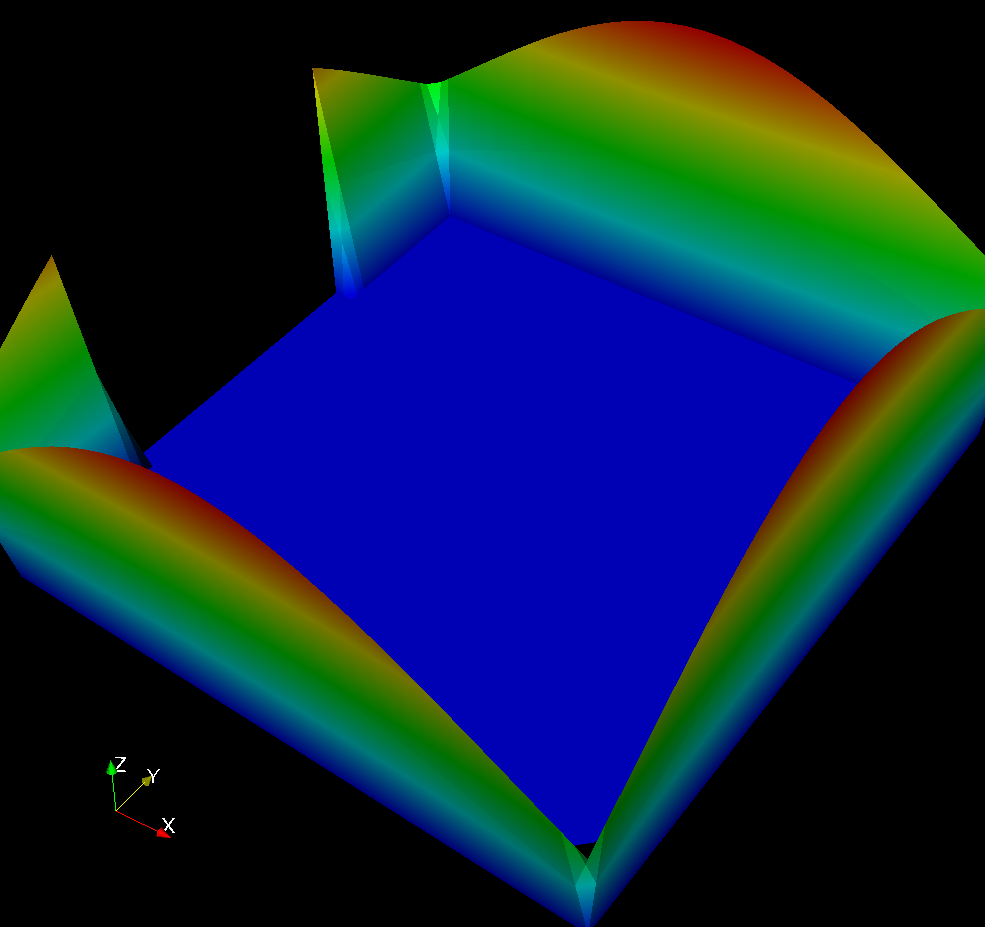
\includegraphics[width=0.65\textwidth]{./EPS/q1constrainedinterpolate}
\end{center}
\end{frame}

Figure \ref{fig:Q1ConstrainedInterpolation} shows the result obtained
after setting the nonconstrained degrees of freedom to zero.


\mode<article>{
\begin{figure}
\begin{center}
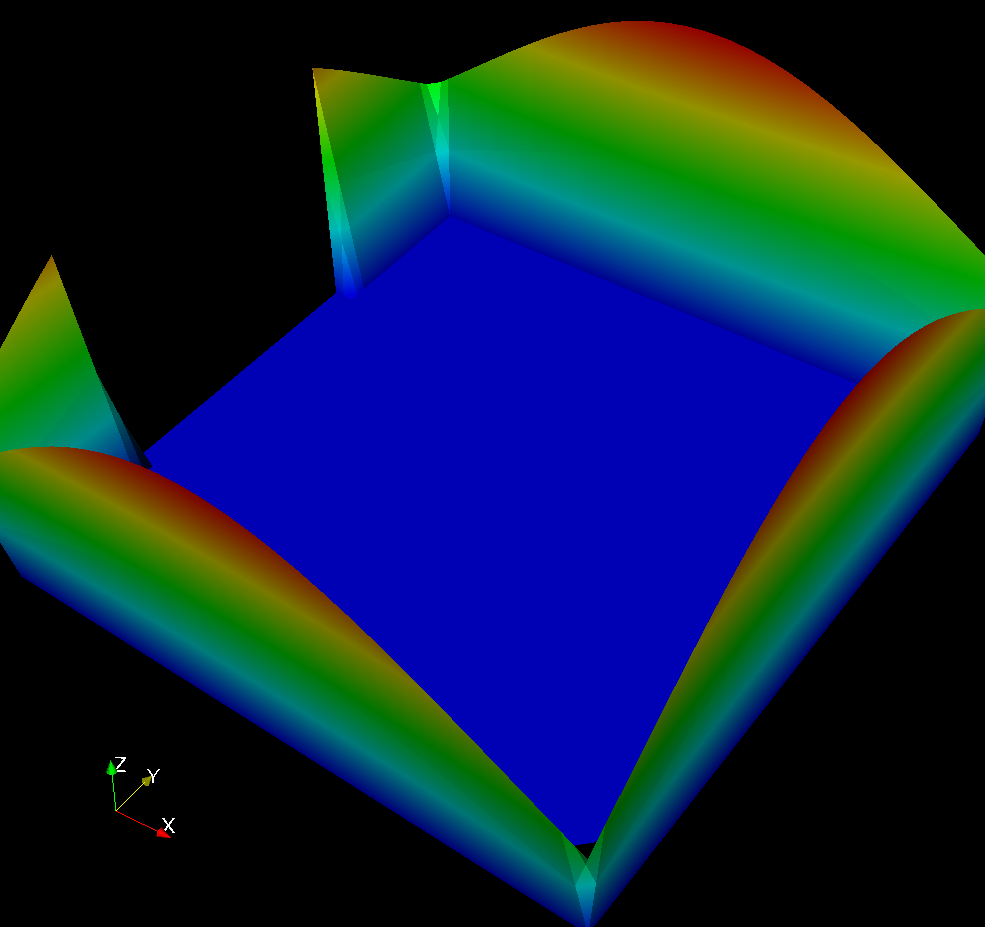
\includegraphics[width=0.5\textwidth]{./EPS/q1constrainedinterpolate}
\end{center}
\caption{Interpolation of $\exp(-3\|x-c\|^2)$ with $Q_1$ elements with
subsequent modification of nonconstrained degrees of freedom.}
\label{fig:Q1ConstrainedInterpolation}
\end{figure}
}


\cleardoublepage

